% Set up the document
\documentclass{article}

% Page size
\usepackage[
    letterpaper,]{geometry}
\usepackage{changepage}

% Lines between paragraphs
\setlength{\parskip}{\baselineskip}
\setlength{\parindent}{0pt}

% Math
\usepackage{mathtools}
\usepackage{amssymb}
\usepackage{amsthm}
\usepackage{commath}

% Shortcut for boldface
\def\*#1{\mathbf{#1}}

% Number sets
\newcommand{\C}{\mathbb{C}}
\newcommand{\N}{\mathbb{N}}
\newcommand{\Q}{\mathbb{Q}}
\newcommand{\R}{\mathbb{R}}
\newcommand{\Z}{\mathbb{Z}}

% Links
\usepackage{hyperref}

% Graphics
\usepackage{float}
\usepackage{graphicx}
\graphicspath{ {./img/} }

% Page numbers at top right
\usepackage{fancyhdr}
\pagestyle{fancy}
\fancyhf{}
\fancyhead[R]{\thepage}
\renewcommand\headrulewidth{0pt}

\begin{document}

\textbf{AMATH 740 assignment 2} \\
\textbf{Matt Wiens} \\
\textbf{2020-09-23}

1. \textbf{Floating point numbers.}
Let $\texttt{eps}$ denote the distance between the number $1$ and
the next floating point number that is greater than $1$. Explain why
(assuming, e.g., IEEE double precision numbers) $\texttt{eps} = 2 \mu$,
where $\mu$ is the unit roundoff of the floating point number system.

\textit{Solution.}
Using the IEEE double precision format
$F(\beta=2,t=53,L=-1022,U=1023)$, we have that if $x = fl(1)$ and
$y$ is the next floating point number greater than $1$ then
%
\begin{align*}
    x &= 1.000 \cdots 000 \cdot 2^0, \\
    y &= 1.000 \cdots 001 \cdot 2^0.
\end{align*}
%
Clearly $\texttt{eps} \coloneqq y - x = 2^{-52}$, but from the course
notes we have that
%
\begin{equation*}
    \mu = \frac{1}{2} \beta^{-t + 1} = \frac{1}{2} 2^{-52}
    ,
\end{equation*}
%
and hence $\texttt{eps} = 2 \mu$.

\newpage

2. \textbf{Rounding errors.}
Consider the expression
%
\begin{equation*}
    z_A = \frac{1}{\sqrt{1 + x^2} - \sqrt{1 - x^2}}.
\end{equation*}
%
(i) Explain why the formula for $z_A$ is susceptible for catastrophic
cancellation errors for $x$ close to $0$.

\textit{Solution.}
The main idea here is that when $x$ is sufficiently small, $x^2 \approx 0$
and so $1 + x^2 \approx 1$ and $1 - x^2 \approx 1$, which can lead to
catastrophic cancellation and a division by zero when computing the expression for $z_A$.

As an example take the floating point system $F(\beta=10,t=5,L=-10,U=10)$
and suppose that $x = 1.0000 \cdot 10^{-3}$. Then
%
\begin{align*}
    fl(1 - x^2) &= fl(1.0000 \cdot 10^0 - 1.0000 \cdot 10^{-6}) = 1.0000 \cdot 10^0, \\
    fl(1 + x^2) &= fl(1.0000 \cdot 10^0 + 1.0000 \cdot 10^{-6}) = 1.0000 \cdot 10^0,
\end{align*}
%
and so the denominator for $z_A$ when computed is $\sqrt{1} - \sqrt{1} = 0$,
which results in a division by zero error.

\vspace{5mm}

(ii) Use reformulation to find an alternative expression $z_B$ for expression
$z_A$ in a way that avoids catastrophic cancellation for $x$ close to $0$.

\textit{Solution.}
We can use a trick of multiplying $z_A$ by $1$ to obtain
%
\begin{align*}
    z_B &=
        \frac{\sqrt{1 + x^2} + \sqrt{1 - x^2}}{\sqrt{1 + x^2} + \sqrt{1 - x^2}}
        z_A \\
        &=
        \frac{\sqrt{1 + x^2} + \sqrt{1 - x^2}}{\sqrt{1 + x^2} + \sqrt{1 - x^2}}
        \frac{1}{\sqrt{1 + x^2} - \sqrt{1 - x^2}}
        \\
        &=
        \frac{\sqrt{1 + x^2} + \sqrt{1 - x^2}}{\sqrt{1 + x^2} + \sqrt{1 - x^2}}
        \frac{1}{\sqrt{1 + x^2} - \sqrt{1 - x^2}}
        \\
        &=
        \frac{\sqrt{1 + x^2} + \sqrt{1 - x^2}}{(1 + x^2) - (1 - x^2)}
        \\
        &=
        \frac{\sqrt{1 + x^2} + \sqrt{1 - x^2}}{2 x^2}
        ,
\end{align*}
%
which avoids catastrophic cancellation when $x$ is close to $0$.

\newpage

3. \textbf{Gram-Schmidt algorithm.}
Consider the matrix
%
\begin{equation*}
    A =
    \begin{bmatrix}
        2 & 0 & 0 \\
        0 & 1 & 1 \\
        0 & 1 & 2 \\
        0 & 0 & 0
    \end{bmatrix}
    .
\end{equation*}
%
(a) Determine (by hand) the reduced $QR$ factorization of $A$ using the
Gram-Schmidt algorithm. That is, orthonormalize the column vectors of $A$,
and write the result as
%
\begin{equation*}
    A = \widehat{Q} \widehat{R},
\end{equation*}
%
with $\widehat{Q} \in \R^{4 \times 3}$ and $\widehat{R} \in \R^{3 \times 3}$. (Keep
the square roots and the divisions by square roots in your answer.)

\textit{Solution.}
First, we determine three orthogonal vectors $\*v_1, \*v_2, \*v_3$ which
span the column space of $A$ (where we denote the columns of $A$ as
$\*a_1, \*a_2, \*a_3$). We take
%
\begin{equation*}
    \*v_1 = \*a_1 = (2, 0, 0, 0)^T
\end{equation*}
%
where $\enVert{\*v_1} = 2$. Then we have
%
\begin{equation*}
    \frac{1}{\enVert{\*v_1}^2} \*v_1^T \*a_2
    = \frac{1}{4} (2, 0, 0, 0) (0, 1, 1, 0)^T = 0
    ,
\end{equation*}
%
and so
%
\begin{equation*}
    \*v_2 = \*a_2 - \frac{1}{\enVert{\*v_1}^2} \*v_1^T \*a_2 \cdot \*v_1
        = \*a_2
        = (0, 1, 1, 0)^T
        ,
\end{equation*}
%
where $\enVert{\*v_2} = \sqrt{2}$. Then, using that
%
\begin{align*}
    \frac{1}{\enVert{\*v_1}^2} \*v_1^T \*a_3
    &= \frac{1}{4} (2, 0, 0, 0) (0, 1, 2, 0)^T = 0, \\
    \frac{1}{\enVert{\*v_2}^2} \*v_2^T \*a_3
    &= \frac{1}{2} (0, 1, 1, 0) (0, 1, 2, 0)^T = \frac{3}{2},
\end{align*}
%
we have
%
\begin{align*}
    \*v_3
        &= \*a_3
            - \frac{1}{\enVert{\*v_1}^2} \*v_1^T \*a_3 \cdot \*v_1
            - \frac{1}{\enVert{\*v_2}^2} \*v_2^T \*a_3 \cdot \*v_2
            \\
        &= \*a_3 - \frac{3}{2} \*v_2
        \\
        &= (0, 1, 2, 0)^T - \frac{3}{2} (0, 1, 1, 0)^T
        \\
        &= \del{0, - \frac{1}{2}, \frac{1}{2}, 0}^T
        ,
\end{align*}
%
where $\enVert{\*v_3} = 1 / \sqrt{2}$.
%
Now, letting $\*q_1, \*q_2, \*q_3$ be the normalized counterparts of $\*v_1, \*v_2, \*v_3$
(that is $\*q_i = \*v_i / \enVert{\*v_i}$ for $i = 1, 2, 3$), we have
%
\begin{align*}
    \*a_1 &= 2 \*q_1, \\
    \*a_2 &= \sqrt{2} \*q_2, \\
    \*a_3 &= \frac{3}{\sqrt{2}} \*q_2 + \frac{1}{\sqrt{2}} \*q_3.
\end{align*}
%
Thus the reduced $QR$ decomposition is given by $A = \widehat{Q} \widehat{R}$ where
%
\begin{equation*}
    \widehat{Q} =
    \begin{bmatrix}
        1 & 0 & 0 \\
        0 & \frac{1}{\sqrt{2}} & - \frac{1}{\sqrt{2}} \\
        0 & \frac{1}{\sqrt{2}} & \frac{1}{\sqrt{2}} \\
        0 & 0 & 0
    \end{bmatrix},
    \quad
    \widehat{R} =
    \begin{bmatrix}
        2 & 0 & 0 \\
        0 & \sqrt{2} & 0 \\
        0 & \frac{3}{\sqrt{2}} & \frac{1}{\sqrt{2}}
    \end{bmatrix}
    .
\end{equation*}

\vspace{5mm}

(b) Extend this to the full $QR$ factorization of $A$,
%
\begin{equation*}
    A = QR,
\end{equation*}
%
with $Q \in \R^{4 \times 4}$ and $R \in \R^{4 \times 3}$. (Keep the square
roots and the divisions by square roots in your answer. Check that the $Q$
you obtain is indeed an orthogonal matrix!)

\textit{Solution.}
For a full $QR$ factorization of $A$, all we need to do is add one additional
unit vector that is orthogonal to the column space of $\widehat{Q}$ to the
columns of $\widehat{Q}$ and append a row of zeros to $\widehat{R}$. The vector
we will add is $(0, 0, 0, 1)^T$; it is easy to see that this is normalized
and orthogonal to the column space of $\widehat{Q}$. Hence we have the $QR$ factorization
$A = QR$ where
%
\begin{equation*}
    Q =
    \begin{bmatrix}
        1 & 0 & 0 & 0 \\
        0 & \frac{1}{\sqrt{2}} & - \frac{1}{\sqrt{2}} & 0\\
        0 & \frac{1}{\sqrt{2}} & \frac{1}{\sqrt{2}} & 0 \\
        0 & 0 & 0 & 1
    \end{bmatrix},
    \quad
    R =
    \begin{bmatrix}
        2 & 0 & 0 \\
        0 & \sqrt{2} & 0 \\
        0 & \frac{3}{\sqrt{2}} & \frac{1}{\sqrt{2}} \\
        0 & 0 & 0
    \end{bmatrix}
    .
\end{equation*}
%
It should be clear from inspection that
%
\begin{equation*}
    Q Q^T = 
    \begin{bmatrix}
        1 & 0 & 0 & 0 \\
        0 & \frac{1}{\sqrt{2}} & - \frac{1}{\sqrt{2}} & 0\\
        0 & \frac{1}{\sqrt{2}} & \frac{1}{\sqrt{2}} & 0 \\
        0 & 0 & 0 & 1
    \end{bmatrix}
    \begin{bmatrix}
        1 & 0 & 0 & 0 \\
        0 & \frac{1}{\sqrt{2}} & \frac{1}{\sqrt{2}} & 0\\
        0 & - \frac{1}{\sqrt{2}} & \frac{1}{\sqrt{2}} & 0 \\
        0 & 0 & 0 & 1
    \end{bmatrix}
    =
    I_4
    .
\end{equation*}

\newpage

4. \textbf{Computational cost of Gram-Schmidt algorithm.}
Let $A \in \R^{m \times n}$ with $m \geq n$. Consider the Gram-Schmidt
algorithm in the lecture notes (Algorithm 3.2). Assuming that both $m$ and
$n$ are large, show that the dominant term in the computational work is given
by
%
\begin{equation*}
    W \approx 2 m n^2 \text{ flops.}
\end{equation*}

\textit{Solution.} First let's determine the cost of each of the steps
inside of loops in the algorithm (the ones that aren't simply assigning values---which
we will assume to be a free operation). For the step
%
\begin{equation*}
    \widehat{r}_{ij} = (\widehat{q}_i)^T a_j
\end{equation*}
%
we are summing over $m$ products. So the cost of this step is $(m - 1) + m = 2m - 1$ flops.

For the step
%
\begin{equation*}
    v_j = v_j - \widehat{r}_{ij} \widehat{q}_i
\end{equation*}
%
we have $m$ products in the right term, and then we take the difference of $m$ terms.
So the cost of this step is $2m$ flops.

For the step
%
\begin{equation*}
    \widehat{r}_{jj} = \enVert{v_j}
\end{equation*}
%
we are taking the square of $m$ terms, summing these terms, and then taking a square root of the sum;
so this too costs $m + (m - 1) + 1 = 2m$ flops.

Finally, for the step
%
\begin{equation*}
    \widehat{q}_j = v_j / r_{jj}
\end{equation*}
%
we are taking $m$ divisions, so this step costs $m$ flops.

Thus considering the loops of Algorithm $3.2.$ in the course notes, we have that the total
work $W$ is given by
%
\begin{align*}
    W &= \sum_{j = 1}^n \sbr{\sum_{i = 1}^{j - 1} \sbr{(2m - 1) + 2m} + 2m + m} \\
      &= \sum_{j = 1}^n \sbr{3m + \sum_{i = 1}^{j - 1} (4m - 1)} \\
      &= 3 mn + (4m - 1) \sum_{j = 1}^n \sum_{i = 1}^{j - 1} 1 \\
      &= 3 mn + (4m - 1) \del{\frac{1}{2} (n - 1) n} \\
      &= 2 mn^2 + m n - \frac{1}{2} n^2 + \frac{1}{2} n
      .
\end{align*}
%
Hence if both $m$ and $n$ are large then the dominant term of the computational cost
is clearly $2 m n^2$.

\newpage

5. \textbf{$\boldsymbol{QR}$ factorization.}
Let
%
\begin{equation*}
    A =
    \begin{bmatrix}
        \*a_1 & \*a_2
    \end{bmatrix}
    =
   \begin{bmatrix}
       4 & 5 \\
       3 & 10
   \end{bmatrix}
   .
\end{equation*}
%
(i) Construct the first Householder reflection matrix, $Q_1$, which reflects
the first column of $A$, $\*a_1$, to a vector
%
\begin{equation*}
    Q_1 \*a_1 =
    \begin{bmatrix}
        \pm \enVert{\*a_1} \\
        0
    \end{bmatrix}
    ;
\end{equation*}
%
that is, choose the sign according to the rule used to ensure numerical
stability, determine the vector $\*v_1$ and its normalized version
$\*u_1$, and then the matrix $Q_1$.

\textit{Solution.}
By inspection we can see that $\enVert{a_1} = 5$. To ensure numerical stability,
we take
%
\begin{equation*}
    Q_1 \*a_1 =
    \begin{bmatrix}
        -5 \\
        0
    \end{bmatrix}
    .
\end{equation*}
%
Then we have the vector $\*v_1$ from $Q_1\*a_1$ to $\*a_1$ given by 
%
\begin{equation*}
    \*v_1 = \*a_1 - Q_1 \*a_1 = (4, 3)^T - (-5, 0)^T = (9, 3)^T
    ,
\end{equation*}
%
which, when normalized, gives
%
\begin{equation*}
    \*u_1
        = \frac{\*v_1}{\enVert{\*v_1}}
        = \frac{1}{3 \sqrt{10}} (9, 3)^T
        = \frac{1}{\sqrt{10}} (3, 1)^T
    .
\end{equation*}
%
Hence, we can calculate $Q_1$ as follows:
%
\begin{align*}
    Q_1
        &= I_2 - 2 \*u_1 \*u_1^T \\
        &= I_2 - 2 \frac{1}{10} (3, 1)^T (3, 1) \\
        &=
        \begin{bmatrix}
            1 & 0 \\
            0 & 1
        \end{bmatrix}
        - \frac{1}{5}
        \begin{bmatrix}
            9 & 3 \\
            3 & 1
        \end{bmatrix}
        \\
        &=
        \frac{1}{5}
        \begin{bmatrix}
            -4 & -3 \\
            -3 & 4
        \end{bmatrix}
\end{align*}

\vspace{5mm}

(ii) Verify that $Q_1$ is an orthogonal matrix.

\textit{Solution.}
To verify that $Q_1$ is orthogonal given our computed matrix, we have
%
\begin{equation*}
    Q_1 Q_1^T = Q_1^2 = \frac{1}{25}
        \begin{bmatrix}
            -4 & -3 \\
            -3 & 4
        \end{bmatrix}
        %
        \begin{bmatrix}
            -4 & -3 \\
            -3 & 4
        \end{bmatrix}
        = \frac{1}{25}
        %
        \begin{bmatrix}
            25 & 0 \\
            0 & 25
        \end{bmatrix}
        = I_2
        .
\end{equation*}

\vspace{5mm}

(iii) Make a sketch in the $\R^2$ plane indicating the vectors
$\*x = (x, y)^T \in \R^2$ that arise in parts (i)--(ii):
the original vector $\*a_1$, and its image $Q_1 \*a_1$ under the reflection.
Also indicate the line about which the vectors are reflected.

\textit{Solution.}
A sketch of $\*a_1$, $Q_1 \*a_1$, and the line of reflection about which
vectors are reflected is shown in Figure~\ref{fig:q5plot}.
%
\begin{figure}
    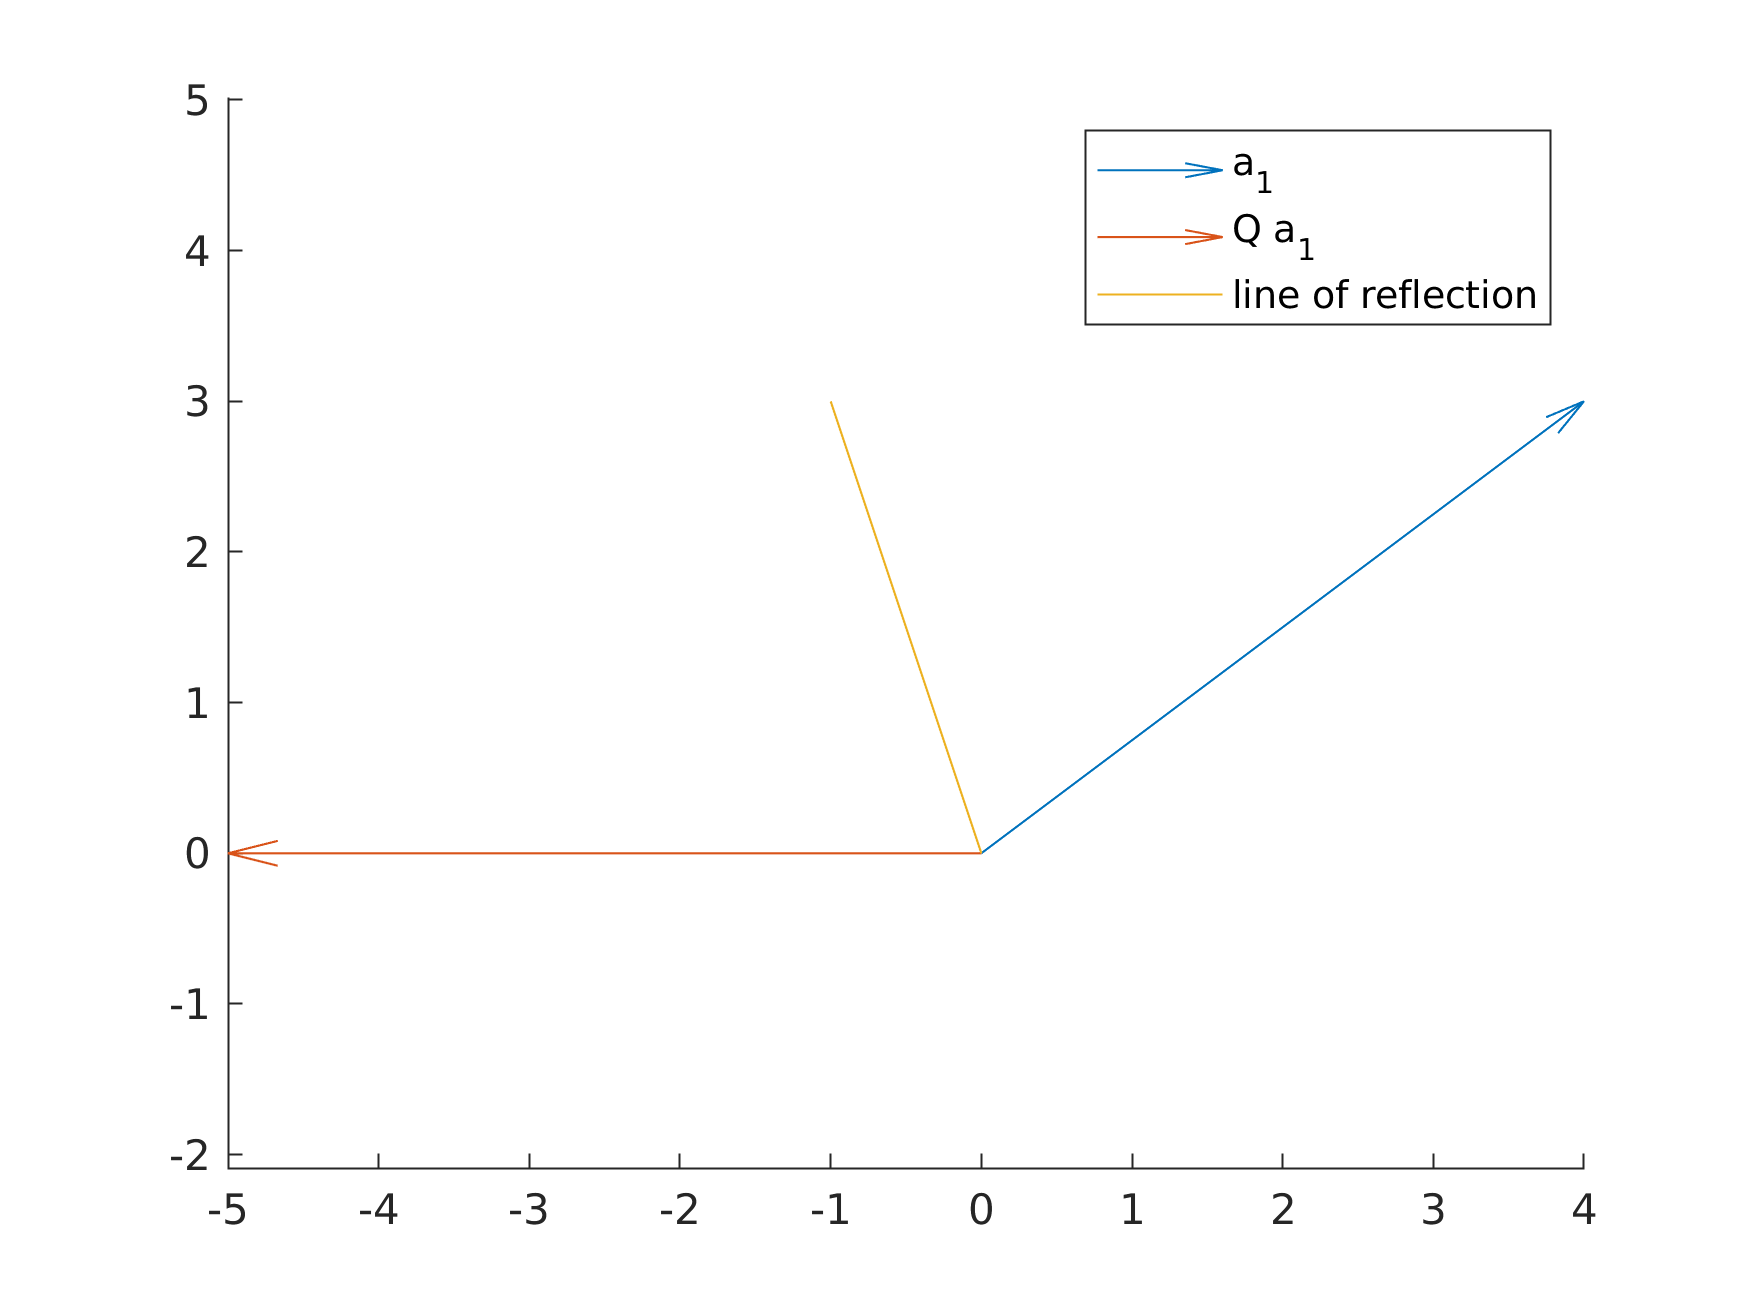
\includegraphics[width=10cm]{q5plot}
    \centering
    \caption{Sketch of Householder elements}
    \label{fig:q5plot}
\end{figure}

\vspace{5mm}

(iv) Compute $Q_1 A$ and write down the $QR$ decomposition of $A$.

\textit{Solution.}
Computing $Q_1 A$ we have
%
\begin{equation*}
    Q_1 A =
        \frac{1}{5}
        \begin{bmatrix}
            -4 & -3 \\
            -3 & 4
        \end{bmatrix}
       \begin{bmatrix}
           4 & 5 \\
           3 & 10
       \end{bmatrix}
       \\ =
        \frac{1}{5}
        \begin{bmatrix}
            -25 & -50 \\
            0 & 25
        \end{bmatrix}
       \\ =
        \begin{bmatrix}
            -5 & -10 \\
            0 & 5
        \end{bmatrix}
\end{equation*}
%
And hence we have that $A = QR$ where $Q = Q_1^{-1} = Q_1^T = Q_1$
and
%
\begin{equation*}
    R =
    \begin{bmatrix}
        -5 & -10 \\
        0 & 5
    \end{bmatrix}
    .
\end{equation*}

\newpage

6. \textbf{Determinant inequality.}
Let $A \in \R^{n \times n}$, and let $a_j$ be the $j$th column of $A$.
Show that
%
\begin{equation*}
    |\det(A)| \leq \prod_{j = 1}^n \enVert{a_j}_2
    .
\end{equation*}

\textit{Solution.}
hint is to use QR decomposition of A and comment is that this question isnt
straightforward

\newpage

7. \textbf{Norm inequality.}
Let $A \in \R^{n \times n}$. Show that if $B \in \R^{n \times n}$ is
singular, then
%
\begin{equation*}
    \frac{\enVert{A - B}}{\enVert{A}} \geq \frac{1}{\kappa(A)}
\end{equation*}
%
for any matrix norm induced by a vector norm.

\textit{Solution.}
hint is to consider a unit vector lying in the nullspace of B and comment
is that this isn't straightforward

\end{document}
